\chapter{Survie}
\label{ch:ch5}

\section{Analyse des variables multi-slices pour la prédiction de la survie}



Dans cette section, nous avons entrepris une analyse approfondie des données \texttt{radiomiques\_multislice.csv} des patients atteints de cancer, dans le but d'identifier les variables les plus pertinentes pour prédire la survie des patients. Notre étude s'est concentrée sur différents types d'injection, à savoir l'ART, le PORT, le TARD et le VEIN, en prenant en considération plusieurs indicateurs mesurés sur une période d'au moins un an. L'objectif principal était de déterminer quelles caractéristiques étaient les plus significatives pour distinguer les patients décédés des patients vivants.

Pour garantir la cohérence de notre échantillon, nous avons inclus uniquement les patients ayant été suivis pendant au moins un an. Cette mesure visait à garantir que les données recueillies étaient représentatives d'une période significative de l'évolution de la maladie.

Pour visualiser les données, nous avons construit des courbes où les numéros de \textit{slice} étaient placés sur l'axe des abscisses et les valeurs des variables sur l'axe des ordonnées. Chaque courbe représente les valeurs d'une variable spécifique pour un patient donné, avec des points reliés pour illustrer l'évolution de cette variable à travers les \textit{slices}.

\begin{figure}[H]
    \centering
    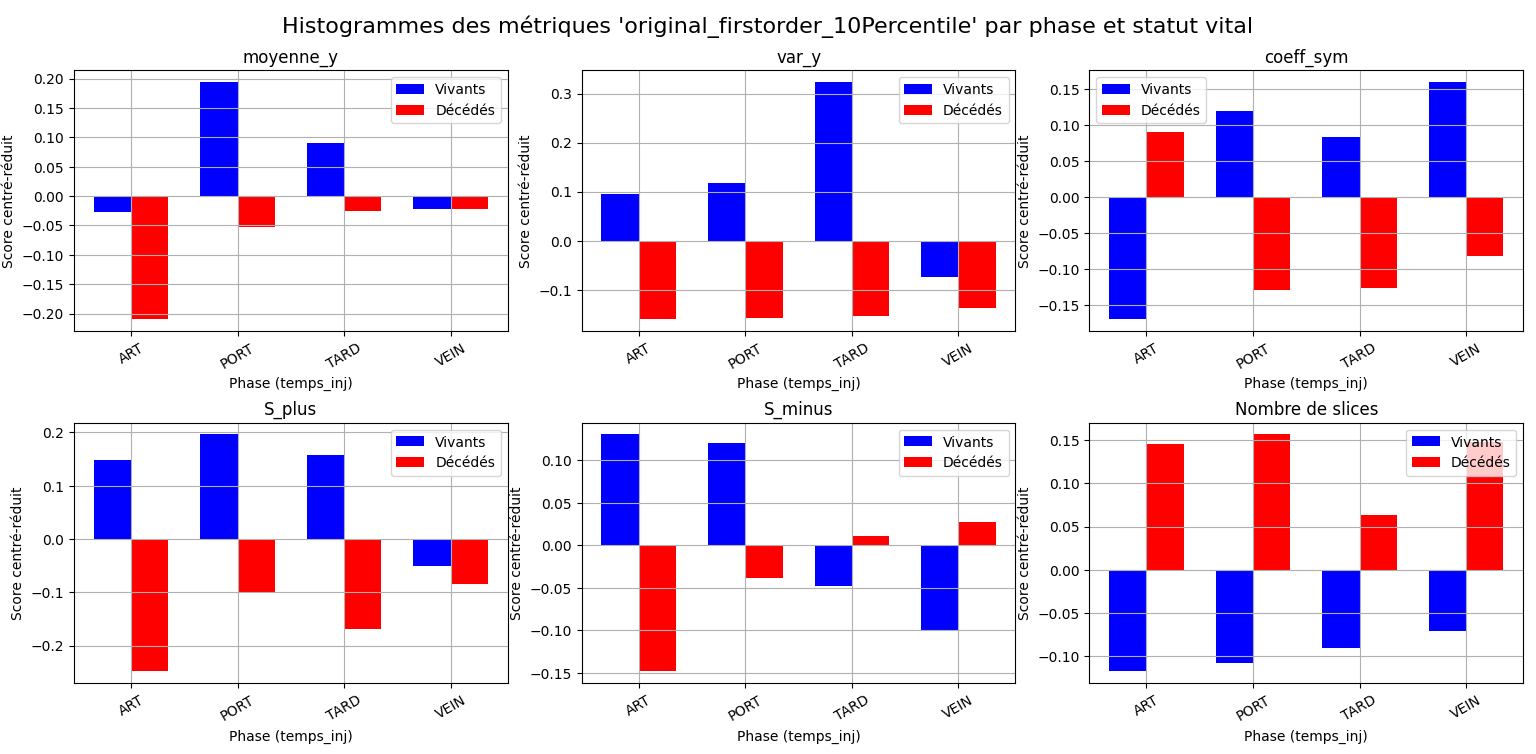
\includegraphics[width=0.45\textwidth]{img/Figure_11.png}
    \caption{Représentation des données de la variable "original\_firstorder\_10Percentile" en fonction du numéro de slices, avec chaque patient représenté par une couleur différente}
\end{figure}


En utilisant ces courbes, nous avons calculé diverses métriques pour chaque patient, notamment :
\begin{itemize}
\item La moyenne des valeurs
\item La variance
\item Le nombre de \textit{slices} par patient
\item L’analyse de la symétrie à l’aide du coefficient d'asymétrie (\textit{skewness})
\item $S^+ = \sum [y_k - y_{k-1}]^+$
\item $S^- = \sum [y_k - y_{k-1}]^-$
\end{itemize}

Après avoir normalisé ces métriques en les centrant et les réduisant, nous avons séparé les patients en deux groupes distincts : les patients décédés et les patients vivants. En calculant les médianes pour chaque métrique et chaque variable dans chaque groupe, nous avons pu évaluer les différences entre les deux populations. Cette approche nous a permis de définir un score pour chaque couple (variable, métrique), représentant la différence absolue entre la médiane des patients décédés et celle des patients vivants :
$$
\scriptstyle \text{Score}(\text{var}, \text{met}) = \left| \text{médiane}_{\text{vivant}}(\text{met}(\text{var})) - \text{médiane}_{\text{mort}}(\text{met}(\text{var})) \right|
$$

Les couples ayant les scores les plus élevés sont considérés comme les plus discriminants.

\begin{figure}[H]
    \centering
    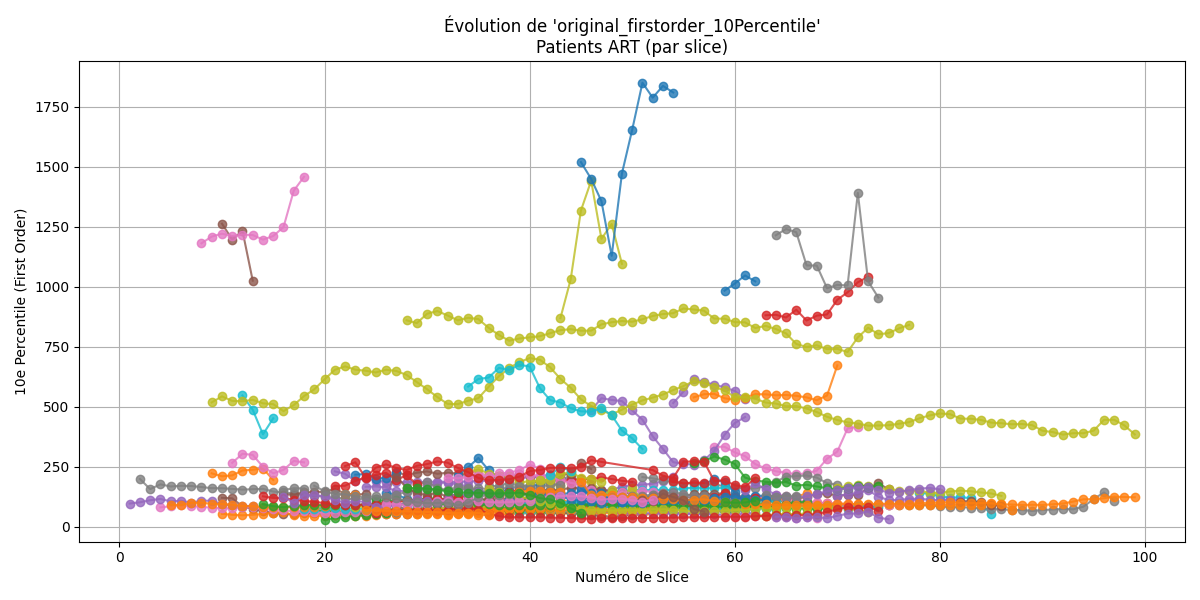
\includegraphics[width=0.4\textwidth]{img/Figure_1.png}
    \caption{Représentation des données de la variable "\texttt{original\_firstorder\_10Percentile}" en fonction du numéro de slices, avec chaque patient représenté par une couleur différente}
\end{figure}


Comme attendu, le nombre de \textit{slices} est une métrique discriminante pour toutes les variables. En effet, un patient ayant une tumeur plus grande a plus de chances d’en décéder qu’un autre.

En ce qui concerne les autres métriques, nous obtenons, comme visible dans l’histogramme ci-contre, des résultats spécifiques à chaque phase d’injection :


\begin{table}[H]
\centering
\tiny{
\begin{tabular}{|c|c|c|}
\hline
\textbf{Phase} & \textbf{Métriques} & \textbf{Variables discriminantes} \\
\hline
ART & $S^+$, variance & original\_glcm\_Idn,  \\
 & & original\_glcm\_Idm,  \\
 & & original\_glcm\_SumEntropy \\
\hline
PORT & variance & original\_glszm\_SmallAreaEmphasis, \\
 & & original\_glrlm\_RunPercentage,  \\
 & & original\_gldm\_SmallDependenceEmphasis, \\
 & & original\_glcm\_Idn \\
\hline
TARD & skewness & original\_firstorder\_Energy,  \\
 & & original\_firstorder\_TotalEnergy, \\
 & & original\_firstorder\_Kurtosis \\
\hline
VEIN & skewness & original\_glrlm\_RunLengthNonUniformityNormalized,  \\
 & & original\_firstorder\_Energy,  \\
 & & original\_firstorder\_Median \\
& $S^+$ & original\_firstorder\_Uniformity \\
\hline
\end{tabular}}
\caption{Couples (métrique, variable) les plus discriminants selon la phase d'injection}
\end{table}
